\chapter{Deep Versat Software Simulator}
\label{chapter:Simulator}

The need for a software simulator comes from the complexity of the configurations being written into Versat and
the hardware simulation faults of being slow.

The goal is to emulate what the hardware is doing much more efficienctly than 
a simple Hardware simulation as the time of development for hardware
is much higher than simple software. The Simulator executes clock iteration per iteration 
getting the same results in each clock as the hardware. As Versat is a CGRA, different functional
unit configurations are easy to accomplish in the simulator and the time to get results on performance
for a specific program is a lot quicker. The only thing the Simualator can't do is predict
if the hardware configurations fits the FPGA that is going to be used and the clocks that 
the hardware can run. But, the propagation time is predictable depending on the number of functional units
as the difference between times in different setups is due to the multiplexers on the inputs of the FUs.

\section{Architecture and Object Relation}

The Simualtor is made up by the Parent Class called Versat, in which will be simulated itself, 
as each Versat instance is independent from each other, the simulations are also independent.
The Versat is made up of 2 CStage Arrays, one is the "live" while the other is the 
shadow registers, where the configurations are held before the simulator is ran.
Each Stage is made up of it's Functional Units, in which each one is connected to the Databus.
As it happens in the hardware, functional units can access the databus which has the output 
of the current stage and previous one.
\clearpage

\begin{figure}[!htbp]
    \centering
    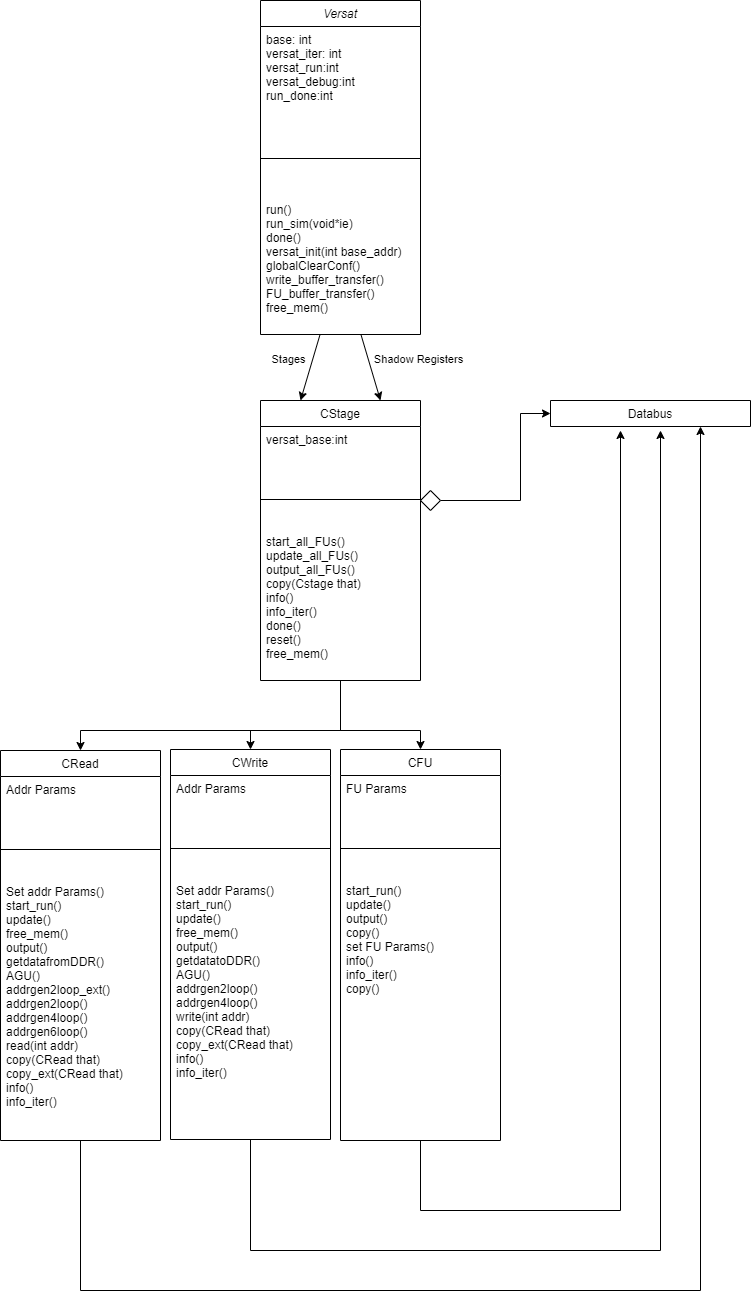
\includegraphics[width=0.8\textwidth]{Figures/VersatSimulatorDraw.drawio.png}
    \caption{Class Structure for the Versat Simulator}
    \label{figure:VersatSimulatorClass}
\end{figure} 

\section{Software API}


%Previously, a software API was made in a previous thesis~\cite{valter:deepversat}
%for Versat. To build on top of this several, software functions were added to make writting configurations to Versat
%easier.

\subsection{Run Simulator}

In the software API for Embedded Versat, the run function would write to a shadow register,
which we can call it "start" changing the value from 0 to 1. Similarly, another register would
change value to 0, which we can call "done". While this last register isn't turned to 1, 
Versat hasn't finished running with the previous configurations so all that can be done is to write
configurations for future runs.

In the simulator, it works in a similar way to preserve compability as the goal is to have the same
programs run on software simulator and on the FPGA.

\lstinputlisting[label=DarknetLiteStrut,language=C++,frame=single,breaklines=true,firstline=222,lastline=245,caption= The Run function code]{./Code/versat.cpp}

As we can see in the previous listing, we reset state variables of the simulator, then shift the 
VO and FU shadow registers.
This is done to simulate the pipeline delay in the FPGA. Because the data needs to come and go to main memory (DDR),
1 run cycle is used just for fetching data and writting data. Using a small example:
If a developer writes a configuration to do a 5x5 matrix multiplication, Versat will have to run 3 times.
Once to fetch data from memory, the second for the actual use of Versat and the final one to get data onto memory.
In the simulator, this is done using the same class instances and copying the configuration values. On the hardware it's several flip-flop registers in a row.
However, all these 3 stages can happen at once if you run multiple configurations in one program, e.g: running a CNN
through Versat, it will have at least 1 run per layer. So, if it has 5 layers, Versat will have to run 5+2 times, the last 2 times are done to
flush the Versat of any data.

After the shift, a new thread is created to run the simulator in parallel with the configurations,
having the same behaviour as the hardware.

\subsection{Simulation Functions}

At the beginning of the configuration run, the method "start_run" of all FUs and memories is started.
This means, for functional units like the Barrel Shifter nothing as it has no delay for the output
\section{Simulation}


